\section{Implementation}

\subsection{Algorithms}

We implemented the stealthy logging mechanism in OpenPLC framework on a Raspberry Pi. The operations in one scan cycle can be described in Algorithm~\ref{logging_algo}. In OpenPLC framework, \textbf{Read\_Input} function and \textbf{Write\_Output} function has been modified to return 1 if any value changes in the current scan cycle. Therefore, only when the input or output values change, this event will be recorded in the log. A single event is encrypted and its key is updated to its hash value, such that the old key for encrypting this event will be overwritten right after each encryption. 

Since the input or output of PLC does not change very often, only reporting changes of input/output values in the log, we can significantly reduce the size of the log. For an application that requires the inputs/outputs of PLCs to be updated very frequently, we suggest to reduce reporting period or ignore some small fluctuations in the analog output.  

After a predefined reporting period is elapsed, the PLC needs to send all the buffered encrypted log to the server and empty the buffer for the next period.

\begin{algorithm}[!t]
\caption{PLC Logging}\label{logging_algo}
\begin{algorithmic}[1]
\Procedure{Logging}{$Period$}
	
	\State $EL = \{\}$
	\State $T = 0$
	\State $Event\_ID = 0$
	\State $Update = 0$
	
	\While{True} \Comment{Scan Cycle}
		\State $Update = 0$
		\State $T = T + 1$
		\State $Update = Read\_Input()$
		\State $PLC\_Logic()$
		\State $Update = Write\_Ouput()$
		\If{$Update == 1 || T \mbox{ mod } Period == 1 $}
			\State $TempLog = \{T, Input, Output, Event\_ID\}$
			\State $EL \gets $(\Call{Encrypt}{$Temp\_Log$, $Key$})
			\State $TempLog = \emptyset$ \Comment{Delete the plaintext}
			\State $Key = $\Call{Hash}{$Key$}
			\State $Event\_ID = Event\_ID + 1$
		\EndIf
		\If{$T\mbox{ mod }Period == 0$}
			\State \Call{Send}{EL}
			\State $EL = \emptyset$ \Comment{Empty the buffer}
			\State $Event\_ID = 0$
		\EndIf
	\EndWhile
\EndProcedure
\end{algorithmic}
\end{algorithm}

The algorithm on the server side works as Algorithm~\ref{server_algo}. The server waits for the incoming packet from the PLC. If the packet is not received on time, the server concludes that the PLC is compromised, we need to restart the PLC. If the server gets the packet on time, then we need to use the associated key to decode this packet and update the key stored at the server. After that, we need to check whether the decrypted data has the correct data format or not. If not, then it means the integrity of the packet has been compromised, we need to restart the PLC. If the integrity is also valid, then we need to extract the input change in this period with its time stamp. This input change and time information is applied to the PLC logic simulator, which will generate the expect output change with its time stamp. Then this expected output is compared with the output received from the PLCs. If they do not match, then the server knows that the logic running on the PLC has been maliciously modified. Therefore, it is also required to restart the PLC in this case.   

\begin{algorithm}[!t]
\caption{Server Monitoring}\label{server_algo}
\begin{algorithmic}[1]
\Procedure{Monitoring}{$Period$}
	
	\State $Alarm = False$
	\State $Last\_Rec\_T = Current\_T$
	
	\While{True}
		\While{True}
			\If {$Current\_T - Last\_Rec\_T > Period$}
				\State $Alarm = True$
				\State Break \Comment{Missing one Packet}
			\EndIf
			\If {$EL \gets$ \Call{Rec\_Packet}}
				\State $Last\_Rec\_T = Current\_T$ 
				\State Break \Comment{Receive one Packet}
			\EndIf
		\EndWhile
		\State $(L, Key) \gets $ \Call{Decrypt\_Packet}{$EL,Key$}
		\State $Alarm \gets $ \Call{Verify\_Format}{$L$}
		\State $(T', Input', Output', Event\_ID') \gets L$
		\State $(T'', Output'') \gets $ \Call{PLC\_Simulate}{$T', Input'$}
		\State $Alarm \gets $ \Call{Compare}{$T', Ouput', T'', Output''$}
		\If {Alarm}
			\State Restart PLC
		\EndIf
	\EndWhile
\EndProcedure
\end{algorithmic}
\end{algorithm}

\subsection{Implementation Details}

As cryptographic primitives, we use AES-128 and SHA-256 as the encryption algorithm and hash function respectively. The updated key is the first 16 bytes of the hash value of the previous key. The reporting period is set to 10 seconds in the prototype implementation, but it can be easily adapted to a different value if it is required by the application. 

To minimize the size of the log we sent, we design one data format to record one event (input or output change) in less than 128 bits, which can fit in one encryption block of AES. The data format is depicted in Figure~\ref{fig:data_format}. The first byte is used as an indicator of the start of one event; we set it as 0xFF. The second and third bytes are used to store the event ID in the current time period. Since the PLC is required to run on 100Hz, and we set the reporting period to be 10 seconds, the maximum of events can happen in one period is 1000. Therefore, two bytes are more than enough to represent the maximum number. The forth and fifth bytes are reserved for device ID. In total, 65536 devices are allowed to be managed by one server. The following 4 bytes are used to store the time stamp, because in OpenPLC framework, it is a 4 byte variable. The next six bytes are divided for storing digital inputs, digital outputs and analog output value respectively. Each of them takes two bytes. Since the number of digital inputs and digital outputs on a Raspberry Pi is 14 and 11. Two bytes are enough to store all the input/output pins. Also, only one analog pin can be used on a Raspberry Pi, and this value can be represented by a 16-bit value stored in 2 bytes. In the end, another byte of 0xFF is appended to indicate the end of one event log. 

\begin{figure*}[h]
  \centering
    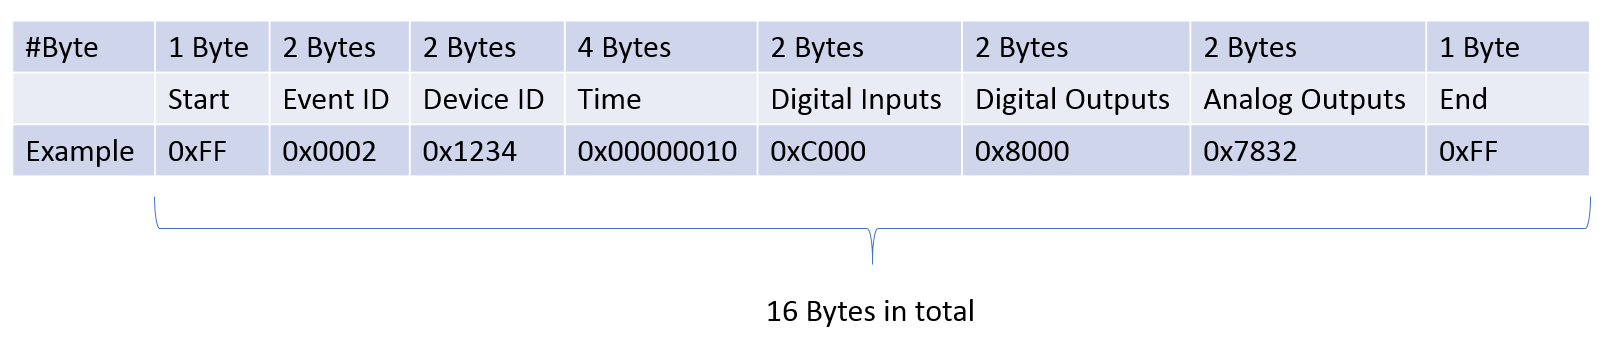
\includegraphics[width=\textwidth]{figs/data_format}
    \caption{Data format of one event in the log.}
    \label{fig:data_format}
\end{figure*}
